\documentclass[twoside]{book}

% Packages required by doxygen
\usepackage{calc}
\usepackage{doxygen}
\usepackage{graphicx}
\usepackage[utf8]{inputenc}
\usepackage{makeidx}
\usepackage{multicol}
\usepackage{multirow}
\usepackage{textcomp}
\usepackage[table]{xcolor}

% Font selection
\usepackage[T1]{fontenc}
\usepackage{mathptmx}
\usepackage[scaled=.90]{helvet}
\usepackage{courier}
\usepackage{amssymb}
\usepackage{sectsty}
\renewcommand{\familydefault}{\sfdefault}
\allsectionsfont{%
  \fontseries{bc}\selectfont%
  \color{darkgray}%
}
\renewcommand{\DoxyLabelFont}{%
  \fontseries{bc}\selectfont%
  \color{darkgray}%
}

% Page & text layout
\usepackage{geometry}
\geometry{%
  a4paper,%
  top=2.5cm,%
  bottom=2.5cm,%
  left=2.5cm,%
  right=2.5cm%
}
\tolerance=750
\hfuzz=15pt
\hbadness=750
\setlength{\emergencystretch}{15pt}
\setlength{\parindent}{0cm}
\setlength{\parskip}{0.2cm}
\makeatletter
\renewcommand{\paragraph}{%
  \@startsection{paragraph}{4}{0ex}{-1.0ex}{1.0ex}{%
    \normalfont\normalsize\bfseries\SS@parafont%
  }%
}
\renewcommand{\subparagraph}{%
  \@startsection{subparagraph}{5}{0ex}{-1.0ex}{1.0ex}{%
    \normalfont\normalsize\bfseries\SS@subparafont%
  }%
}
\makeatother

% Headers & footers
\usepackage{fancyhdr}
\pagestyle{fancyplain}
\fancyhead[LE]{\fancyplain{}{\bfseries\thepage}}
\fancyhead[CE]{\fancyplain{}{}}
\fancyhead[RE]{\fancyplain{}{\bfseries\leftmark}}
\fancyhead[LO]{\fancyplain{}{\bfseries\rightmark}}
\fancyhead[CO]{\fancyplain{}{}}
\fancyhead[RO]{\fancyplain{}{\bfseries\thepage}}
\fancyfoot[LE]{\fancyplain{}{}}
\fancyfoot[CE]{\fancyplain{}{}}
\fancyfoot[RE]{\fancyplain{}{\bfseries\scriptsize Generated on Sun Apr 16 2017 13\-:52\-:32 for My Project by Doxygen }}
\fancyfoot[LO]{\fancyplain{}{\bfseries\scriptsize Generated on Sun Apr 16 2017 13\-:52\-:32 for My Project by Doxygen }}
\fancyfoot[CO]{\fancyplain{}{}}
\fancyfoot[RO]{\fancyplain{}{}}
\renewcommand{\footrulewidth}{0.4pt}
\renewcommand{\chaptermark}[1]{%
  \markboth{#1}{}%
}
\renewcommand{\sectionmark}[1]{%
  \markright{\thesection\ #1}%
}

% Indices & bibliography
\usepackage{natbib}
\usepackage[titles]{tocloft}
\setcounter{tocdepth}{3}
\setcounter{secnumdepth}{5}
\makeindex

% Hyperlinks (required, but should be loaded last)
\usepackage{ifpdf}
\ifpdf
  \usepackage[pdftex,pagebackref=true]{hyperref}
\else
  \usepackage[ps2pdf,pagebackref=true]{hyperref}
\fi
\hypersetup{%
  colorlinks=true,%
  linkcolor=blue,%
  citecolor=blue,%
  unicode%
}

% Custom commands
\newcommand{\clearemptydoublepage}{%
  \newpage{\pagestyle{empty}\cleardoublepage}%
}


%===== C O N T E N T S =====

\begin{document}

% Titlepage & ToC
\hypersetup{pageanchor=false}
\pagenumbering{roman}
\begin{titlepage}
\vspace*{7cm}
\begin{center}%
{\Large My Project }\\
\vspace*{1cm}
{\large Generated by Doxygen 1.8.6}\\
\vspace*{0.5cm}
{\small Sun Apr 16 2017 13:52:32}\\
\end{center}
\end{titlepage}
\clearemptydoublepage
\tableofcontents
\clearemptydoublepage
\pagenumbering{arabic}
\hypersetup{pageanchor=true}

%--- Begin generated contents ---
\chapter{Hierarchical Index}
\section{Class Hierarchy}
This inheritance list is sorted roughly, but not completely, alphabetically\-:\begin{DoxyCompactList}
\item \contentsline{section}{Binary\-Search\-Tree$<$ Key, Value $>$}{\pageref{classBinarySearchTree}}{}
\begin{DoxyCompactList}
\item \contentsline{section}{A\-V\-L\-Tree$<$ Key, Value $>$}{\pageref{classAVLTree}}{}
\end{DoxyCompactList}
\item \contentsline{section}{Binary\-Search\-Tree$<$ int, int $>$}{\pageref{classBinarySearchTree}}{}
\item \contentsline{section}{Binary\-Search\-Tree$<$ Key, Value $>$\-:\-:iterator}{\pageref{classBinarySearchTree_1_1iterator}}{}
\item \contentsline{section}{Node$<$ Key, Value $>$}{\pageref{classNode}}{}
\begin{DoxyCompactList}
\item \contentsline{section}{A\-V\-L\-Node$<$ Key, Value $>$}{\pageref{classAVLNode}}{}
\end{DoxyCompactList}
\item \contentsline{section}{Node$<$ int, int $>$}{\pageref{classNode}}{}
\item \contentsline{section}{Rectangle}{\pageref{structRectangle}}{}
\item Test\begin{DoxyCompactList}
\item \contentsline{section}{Tree\-Test}{\pageref{classTreeTest}}{}
\end{DoxyCompactList}
\end{DoxyCompactList}

\chapter{Class Index}
\section{Class List}
Here are the classes, structs, unions and interfaces with brief descriptions\-:\begin{DoxyCompactList}
\item\contentsline{section}{\hyperlink{classAVLNode}{A\-V\-L\-Node$<$ Key, Value $>$} }{\pageref{classAVLNode}}{}
\item\contentsline{section}{\hyperlink{classAVLTree}{A\-V\-L\-Tree$<$ Key, Value $>$} }{\pageref{classAVLTree}}{}
\item\contentsline{section}{\hyperlink{classBinarySearchTree}{Binary\-Search\-Tree$<$ Key, Value $>$} }{\pageref{classBinarySearchTree}}{}
\item\contentsline{section}{\hyperlink{classBinarySearchTree_1_1iterator}{Binary\-Search\-Tree$<$ Key, Value $>$\-::iterator} }{\pageref{classBinarySearchTree_1_1iterator}}{}
\item\contentsline{section}{\hyperlink{classNode}{Node$<$ Key, Value $>$} }{\pageref{classNode}}{}
\item\contentsline{section}{\hyperlink{structRectangle}{Rectangle} }{\pageref{structRectangle}}{}
\item\contentsline{section}{\hyperlink{classTreeTest}{Tree\-Test} }{\pageref{classTreeTest}}{}
\end{DoxyCompactList}

\chapter{Class Documentation}
\hypertarget{classAVLNode}{\section{A\-V\-L\-Node$<$ Key, Value $>$ Class Template Reference}
\label{classAVLNode}\index{A\-V\-L\-Node$<$ Key, Value $>$@{A\-V\-L\-Node$<$ Key, Value $>$}}
}


{\ttfamily \#include $<$avlbst.\-h$>$}

Inheritance diagram for A\-V\-L\-Node$<$ Key, Value $>$\-:\begin{figure}[H]
\begin{center}
\leavevmode
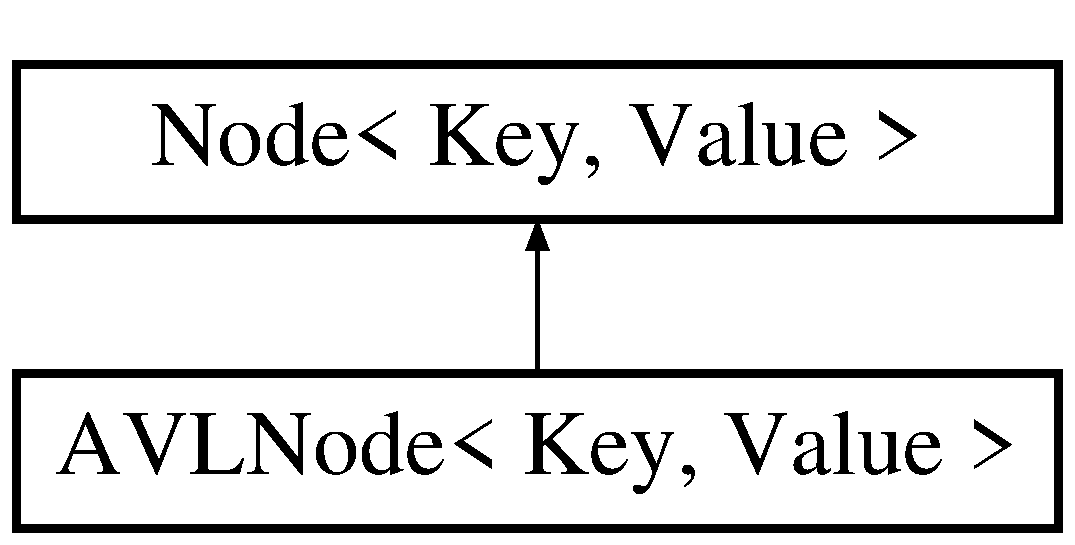
\includegraphics[height=2.000000cm]{classAVLNode}
\end{center}
\end{figure}
\subsection*{Public Member Functions}
\begin{DoxyCompactItemize}
\item 
\hyperlink{classAVLNode_a0c590cfe936353fe4d6eca380747d2d7}{A\-V\-L\-Node} (const Key \&key, const Value \&value, \hyperlink{classAVLNode}{A\-V\-L\-Node}$<$ Key, Value $>$ $\ast$parent)
\item 
virtual \hyperlink{classAVLNode_aaa13278d912e6dbd1147973213b61ec2}{$\sim$\-A\-V\-L\-Node} ()
\item 
char \hyperlink{classAVLNode_a98998d2f9be815c9775dddd0cf950a9a}{get\-Balance} () const 
\item 
void \hyperlink{classAVLNode_a5edf25a95b444da26b20ad1546ac31a9}{set\-Balance} (char balance)
\item 
void \hyperlink{classAVLNode_aa2bc7512704adb240d8e1c18c1c15853}{update\-Balance} (char diff)
\item 
virtual \hyperlink{classAVLNode}{A\-V\-L\-Node}$<$ Key, Value $>$ $\ast$ \hyperlink{classAVLNode_a192664222857753573eba15c6e9b6205}{get\-Parent} () const override
\item 
virtual \hyperlink{classAVLNode}{A\-V\-L\-Node}$<$ Key, Value $>$ $\ast$ \hyperlink{classAVLNode_af681acf83cebd11fb1083262b8100c70}{get\-Left} () const override
\item 
virtual \hyperlink{classAVLNode}{A\-V\-L\-Node}$<$ Key, Value $>$ $\ast$ \hyperlink{classAVLNode_ac57cebda2c1b448d22e00dcb9248cfb8}{get\-Right} () const override
\end{DoxyCompactItemize}
\subsection*{Protected Attributes}
\begin{DoxyCompactItemize}
\item 
\hypertarget{classAVLNode_afa3bbeb9d7bc41b5fee49c23d5bb298a}{char {\bfseries balance\-\_\-}}\label{classAVLNode_afa3bbeb9d7bc41b5fee49c23d5bb298a}

\end{DoxyCompactItemize}


\subsection{Detailed Description}
\subsubsection*{template$<$typename Key, typename Value$>$class A\-V\-L\-Node$<$ Key, Value $>$}

A special kind of node for an A\-V\-L tree, which adds the balance as a data member, plus other additional helper functions. You do N\-O\-T need to implement any functionality or add additional data members or helper functions. 

\subsection{Constructor \& Destructor Documentation}
\hypertarget{classAVLNode_a0c590cfe936353fe4d6eca380747d2d7}{\index{A\-V\-L\-Node@{A\-V\-L\-Node}!A\-V\-L\-Node@{A\-V\-L\-Node}}
\index{A\-V\-L\-Node@{A\-V\-L\-Node}!AVLNode@{A\-V\-L\-Node}}
\subsubsection[{A\-V\-L\-Node}]{\setlength{\rightskip}{0pt plus 5cm}template$<$typename Key , typename Value $>$ {\bf A\-V\-L\-Node}$<$ Key, Value $>$\-::{\bf A\-V\-L\-Node} (
\begin{DoxyParamCaption}
\item[{const Key \&}]{key, }
\item[{const Value \&}]{value, }
\item[{{\bf A\-V\-L\-Node}$<$ Key, Value $>$ $\ast$}]{parent}
\end{DoxyParamCaption}
)}}\label{classAVLNode_a0c590cfe936353fe4d6eca380747d2d7}
Constructor for an \hyperlink{classAVLNode}{A\-V\-L\-Node}. Nodes are initialized with a balance of 0. \hypertarget{classAVLNode_aaa13278d912e6dbd1147973213b61ec2}{\index{A\-V\-L\-Node@{A\-V\-L\-Node}!$\sim$\-A\-V\-L\-Node@{$\sim$\-A\-V\-L\-Node}}
\index{$\sim$\-A\-V\-L\-Node@{$\sim$\-A\-V\-L\-Node}!AVLNode@{A\-V\-L\-Node}}
\subsubsection[{$\sim$\-A\-V\-L\-Node}]{\setlength{\rightskip}{0pt plus 5cm}template$<$typename Key , typename Value $>$ {\bf A\-V\-L\-Node}$<$ Key, Value $>$\-::$\sim${\bf A\-V\-L\-Node} (
\begin{DoxyParamCaption}
{}
\end{DoxyParamCaption}
)\hspace{0.3cm}{\ttfamily [virtual]}}}\label{classAVLNode_aaa13278d912e6dbd1147973213b61ec2}
Destructor. 

\subsection{Member Function Documentation}
\hypertarget{classAVLNode_a98998d2f9be815c9775dddd0cf950a9a}{\index{A\-V\-L\-Node@{A\-V\-L\-Node}!get\-Balance@{get\-Balance}}
\index{get\-Balance@{get\-Balance}!AVLNode@{A\-V\-L\-Node}}
\subsubsection[{get\-Balance}]{\setlength{\rightskip}{0pt plus 5cm}template$<$class Key , class Value $>$ char {\bf A\-V\-L\-Node}$<$ Key, Value $>$\-::get\-Balance (
\begin{DoxyParamCaption}
{}
\end{DoxyParamCaption}
) const}}\label{classAVLNode_a98998d2f9be815c9775dddd0cf950a9a}
A getter for the balance of a \hyperlink{classAVLNode}{A\-V\-L\-Node}. \hypertarget{classAVLNode_af681acf83cebd11fb1083262b8100c70}{\index{A\-V\-L\-Node@{A\-V\-L\-Node}!get\-Left@{get\-Left}}
\index{get\-Left@{get\-Left}!AVLNode@{A\-V\-L\-Node}}
\subsubsection[{get\-Left}]{\setlength{\rightskip}{0pt plus 5cm}template$<$typename Key , typename Value $>$ {\bf A\-V\-L\-Node}$<$ Key, Value $>$ $\ast$ {\bf A\-V\-L\-Node}$<$ Key, Value $>$\-::get\-Left (
\begin{DoxyParamCaption}
{}
\end{DoxyParamCaption}
) const\hspace{0.3cm}{\ttfamily [override]}, {\ttfamily [virtual]}}}\label{classAVLNode_af681acf83cebd11fb1083262b8100c70}
Getter function for the left child. Used since the node inherits from a base node. 

Reimplemented from \hyperlink{classNode_a2c142346d13ce08214ebee5ab76fbf72}{Node$<$ Key, Value $>$}.

\hypertarget{classAVLNode_a192664222857753573eba15c6e9b6205}{\index{A\-V\-L\-Node@{A\-V\-L\-Node}!get\-Parent@{get\-Parent}}
\index{get\-Parent@{get\-Parent}!AVLNode@{A\-V\-L\-Node}}
\subsubsection[{get\-Parent}]{\setlength{\rightskip}{0pt plus 5cm}template$<$typename Key , typename Value $>$ {\bf A\-V\-L\-Node}$<$ Key, Value $>$ $\ast$ {\bf A\-V\-L\-Node}$<$ Key, Value $>$\-::get\-Parent (
\begin{DoxyParamCaption}
{}
\end{DoxyParamCaption}
) const\hspace{0.3cm}{\ttfamily [override]}, {\ttfamily [virtual]}}}\label{classAVLNode_a192664222857753573eba15c6e9b6205}
Getter function for the parent. Used since the node inherits from a base node. 

Reimplemented from \hyperlink{classNode_a89780f3166c5d3aad0bd2960ce65f7a8}{Node$<$ Key, Value $>$}.

\hypertarget{classAVLNode_ac57cebda2c1b448d22e00dcb9248cfb8}{\index{A\-V\-L\-Node@{A\-V\-L\-Node}!get\-Right@{get\-Right}}
\index{get\-Right@{get\-Right}!AVLNode@{A\-V\-L\-Node}}
\subsubsection[{get\-Right}]{\setlength{\rightskip}{0pt plus 5cm}template$<$typename Key , typename Value $>$ {\bf A\-V\-L\-Node}$<$ Key, Value $>$ $\ast$ {\bf A\-V\-L\-Node}$<$ Key, Value $>$\-::get\-Right (
\begin{DoxyParamCaption}
{}
\end{DoxyParamCaption}
) const\hspace{0.3cm}{\ttfamily [override]}, {\ttfamily [virtual]}}}\label{classAVLNode_ac57cebda2c1b448d22e00dcb9248cfb8}
Getter function for the right child. Used since the node inherits from a base node. 

Reimplemented from \hyperlink{classNode_ae9aabb17b3555af256dc9ae091c0bb39}{Node$<$ Key, Value $>$}.

\hypertarget{classAVLNode_a5edf25a95b444da26b20ad1546ac31a9}{\index{A\-V\-L\-Node@{A\-V\-L\-Node}!set\-Balance@{set\-Balance}}
\index{set\-Balance@{set\-Balance}!AVLNode@{A\-V\-L\-Node}}
\subsubsection[{set\-Balance}]{\setlength{\rightskip}{0pt plus 5cm}template$<$class Key , class Value $>$ void {\bf A\-V\-L\-Node}$<$ Key, Value $>$\-::set\-Balance (
\begin{DoxyParamCaption}
\item[{char}]{balance}
\end{DoxyParamCaption}
)}}\label{classAVLNode_a5edf25a95b444da26b20ad1546ac31a9}
A setter for the balance of a \hyperlink{classAVLNode}{A\-V\-L\-Node}. \hypertarget{classAVLNode_aa2bc7512704adb240d8e1c18c1c15853}{\index{A\-V\-L\-Node@{A\-V\-L\-Node}!update\-Balance@{update\-Balance}}
\index{update\-Balance@{update\-Balance}!AVLNode@{A\-V\-L\-Node}}
\subsubsection[{update\-Balance}]{\setlength{\rightskip}{0pt plus 5cm}template$<$class Key , class Value $>$ void {\bf A\-V\-L\-Node}$<$ Key, Value $>$\-::update\-Balance (
\begin{DoxyParamCaption}
\item[{char}]{diff}
\end{DoxyParamCaption}
)}}\label{classAVLNode_aa2bc7512704adb240d8e1c18c1c15853}
Adds diff to the balance of a \hyperlink{classAVLNode}{A\-V\-L\-Node}. 

The documentation for this class was generated from the following file\-:\begin{DoxyCompactItemize}
\item 
avlbst.\-h\end{DoxyCompactItemize}

\hypertarget{classAVLTree}{\section{A\-V\-L\-Tree$<$ Key, Value $>$ Class Template Reference}
\label{classAVLTree}\index{A\-V\-L\-Tree$<$ Key, Value $>$@{A\-V\-L\-Tree$<$ Key, Value $>$}}
}


{\ttfamily \#include $<$avlbst.\-h$>$}

Inheritance diagram for A\-V\-L\-Tree$<$ Key, Value $>$\-:\begin{figure}[H]
\begin{center}
\leavevmode
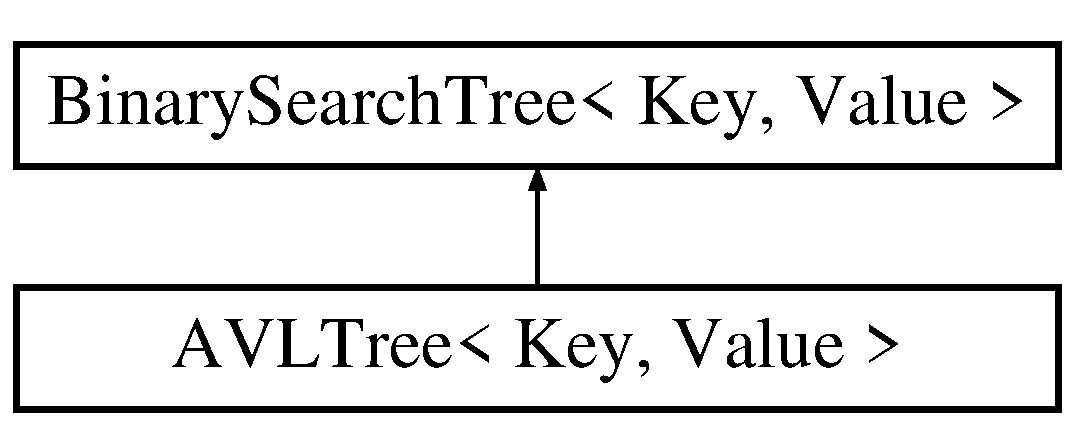
\includegraphics[height=2.000000cm]{classAVLTree}
\end{center}
\end{figure}
\subsection*{Public Member Functions}
\begin{DoxyCompactItemize}
\item 
virtual void \hyperlink{classAVLTree_a7a133667454794bc8fe84beb91fc7f9a}{insert} (const std\-::pair$<$ Key, Value $>$ \&key\-Value\-Pair) override
\item 
virtual void \hyperlink{classAVLTree_a52c0c85de9cbd8f0d30853fc8a853014}{erase} (const Key \&key)
\end{DoxyCompactItemize}
\subsection*{Additional Inherited Members}


\subsection{Detailed Description}
\subsubsection*{template$<$class Key, class Value$>$class A\-V\-L\-Tree$<$ Key, Value $>$}

A templated balanced binary search tree implemented as an A\-V\-L tree. 

\subsection{Member Function Documentation}
\hypertarget{classAVLTree_a52c0c85de9cbd8f0d30853fc8a853014}{\index{A\-V\-L\-Tree@{A\-V\-L\-Tree}!erase@{erase}}
\index{erase@{erase}!AVLTree@{A\-V\-L\-Tree}}
\subsubsection[{erase}]{\setlength{\rightskip}{0pt plus 5cm}template$<$typename Key , typename Value $>$ void {\bf A\-V\-L\-Tree}$<$ Key, Value $>$\-::erase (
\begin{DoxyParamCaption}
\item[{const Key \&}]{key}
\end{DoxyParamCaption}
)\hspace{0.3cm}{\ttfamily [virtual]}}}\label{classAVLTree_a52c0c85de9cbd8f0d30853fc8a853014}
Erase function for a given key. Finds the node, reattaches pointers, and then balances when finished. \hypertarget{classAVLTree_a7a133667454794bc8fe84beb91fc7f9a}{\index{A\-V\-L\-Tree@{A\-V\-L\-Tree}!insert@{insert}}
\index{insert@{insert}!AVLTree@{A\-V\-L\-Tree}}
\subsubsection[{insert}]{\setlength{\rightskip}{0pt plus 5cm}template$<$typename Key , typename Value $>$ void {\bf A\-V\-L\-Tree}$<$ Key, Value $>$\-::insert (
\begin{DoxyParamCaption}
\item[{const std\-::pair$<$ Key, Value $>$ \&}]{key\-Value\-Pair}
\end{DoxyParamCaption}
)\hspace{0.3cm}{\ttfamily [override]}, {\ttfamily [virtual]}}}\label{classAVLTree_a7a133667454794bc8fe84beb91fc7f9a}
Insert function for a key value pair. Finds location to insert the node and then balances the tree. 

Reimplemented from \hyperlink{classBinarySearchTree_af78f03f88b44453dc2e35278c49b2965}{Binary\-Search\-Tree$<$ Key, Value $>$}.



The documentation for this class was generated from the following file\-:\begin{DoxyCompactItemize}
\item 
avlbst.\-h\end{DoxyCompactItemize}

\hypertarget{classBinarySearchTree}{\section{Binary\-Search\-Tree$<$ Key, Value $>$ Class Template Reference}
\label{classBinarySearchTree}\index{Binary\-Search\-Tree$<$ Key, Value $>$@{Binary\-Search\-Tree$<$ Key, Value $>$}}
}


{\ttfamily \#include $<$bst.\-h$>$}

Inheritance diagram for Binary\-Search\-Tree$<$ Key, Value $>$\-:\begin{figure}[H]
\begin{center}
\leavevmode
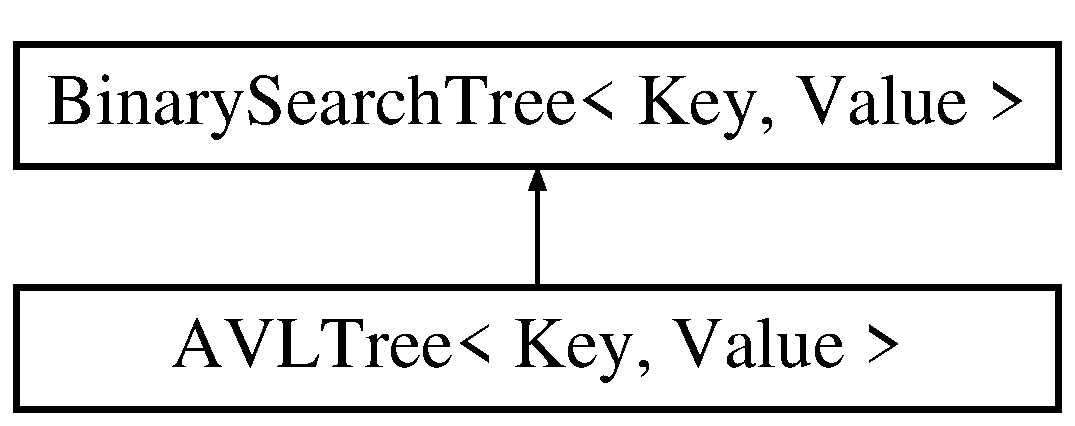
\includegraphics[height=2.000000cm]{classBinarySearchTree}
\end{center}
\end{figure}
\subsection*{Classes}
\begin{DoxyCompactItemize}
\item 
class \hyperlink{classBinarySearchTree_1_1iterator}{iterator}
\end{DoxyCompactItemize}
\subsection*{Public Member Functions}
\begin{DoxyCompactItemize}
\item 
\hyperlink{classBinarySearchTree_ad755ed0485364094f462ce45cf6ecf62}{Binary\-Search\-Tree} ()
\item 
virtual void \hyperlink{classBinarySearchTree_af78f03f88b44453dc2e35278c49b2965}{insert} (const std\-::pair$<$ Key, Value $>$ \&key\-Value\-Pair)
\item 
void \hyperlink{classBinarySearchTree_acce1030d8eb99522591b90e0824e7bbc}{clear} ()
\item 
\hypertarget{classBinarySearchTree_af2f724b66e0da79f2d65144824224c97}{void {\bfseries print} () const }\label{classBinarySearchTree_af2f724b66e0da79f2d65144824224c97}

\item 
\hyperlink{classBinarySearchTree_1_1iterator}{iterator} \hyperlink{classBinarySearchTree_ac42b6e11e290cf9eaf56eba56ca56818}{begin} ()
\item 
\hyperlink{classBinarySearchTree_1_1iterator}{iterator} \hyperlink{classBinarySearchTree_a6603b43057a4bf2843381b8abcb0d010}{end} ()
\item 
\hyperlink{classBinarySearchTree_1_1iterator}{iterator} \hyperlink{classBinarySearchTree_a43958308bfdd55c71cb926d32816f3c1}{find} (const Key \&key) const 
\end{DoxyCompactItemize}
\subsection*{Public Attributes}
\begin{DoxyCompactItemize}
\item 
\hypertarget{classBinarySearchTree_a86747f59a7d863080da23a74bea8ed1c}{\hyperlink{classNode}{Node}$<$ Key, Value $>$ $\ast$ {\bfseries m\-Root}}\label{classBinarySearchTree_a86747f59a7d863080da23a74bea8ed1c}

\end{DoxyCompactItemize}
\subsection*{Protected Member Functions}
\begin{DoxyCompactItemize}
\item 
\hyperlink{classNode}{Node}$<$ Key, Value $>$ $\ast$ \hyperlink{classBinarySearchTree_af7b5e0c65afb9034c2363a6f6a132e39}{internal\-Find} (const Key \&key) const 
\item 
void \hyperlink{classBinarySearchTree_a45a1345e1d2bd7a2a0fdec9298ef8c18}{print\-Root} (\hyperlink{classNode}{Node}$<$ Key, Value $>$ $\ast$root) const 
\item 
void \hyperlink{classBinarySearchTree_ad32ddc43ed2e2464cc0eb6449d2dac40}{delete\-All} (\hyperlink{classNode}{Node}$<$ Key, Value $>$ $\ast$root)
\end{DoxyCompactItemize}


\subsection{Detailed Description}
\subsubsection*{template$<$typename Key, typename Value$>$class Binary\-Search\-Tree$<$ Key, Value $>$}

A templated unbalanced binary search tree. 

\subsection{Constructor \& Destructor Documentation}
\hypertarget{classBinarySearchTree_ad755ed0485364094f462ce45cf6ecf62}{\index{Binary\-Search\-Tree@{Binary\-Search\-Tree}!Binary\-Search\-Tree@{Binary\-Search\-Tree}}
\index{Binary\-Search\-Tree@{Binary\-Search\-Tree}!BinarySearchTree@{Binary\-Search\-Tree}}
\subsubsection[{Binary\-Search\-Tree}]{\setlength{\rightskip}{0pt plus 5cm}template$<$typename Key , typename Value $>$ {\bf Binary\-Search\-Tree}$<$ Key, Value $>$\-::{\bf Binary\-Search\-Tree} (
\begin{DoxyParamCaption}
{}
\end{DoxyParamCaption}
)}}\label{classBinarySearchTree_ad755ed0485364094f462ce45cf6ecf62}
Default constructor for a \hyperlink{classBinarySearchTree}{Binary\-Search\-Tree}, which sets the root to N\-U\-L\-L. 

\subsection{Member Function Documentation}
\hypertarget{classBinarySearchTree_ac42b6e11e290cf9eaf56eba56ca56818}{\index{Binary\-Search\-Tree@{Binary\-Search\-Tree}!begin@{begin}}
\index{begin@{begin}!BinarySearchTree@{Binary\-Search\-Tree}}
\subsubsection[{begin}]{\setlength{\rightskip}{0pt plus 5cm}template$<$typename Key , typename Value $>$ {\bf Binary\-Search\-Tree}$<$ Key, Value $>$\-::{\bf iterator} {\bf Binary\-Search\-Tree}$<$ Key, Value $>$\-::begin (
\begin{DoxyParamCaption}
{}
\end{DoxyParamCaption}
)}}\label{classBinarySearchTree_ac42b6e11e290cf9eaf56eba56ca56818}
Returns an iterator to the \char`\"{}smallest\char`\"{} item in the tree \hypertarget{classBinarySearchTree_acce1030d8eb99522591b90e0824e7bbc}{\index{Binary\-Search\-Tree@{Binary\-Search\-Tree}!clear@{clear}}
\index{clear@{clear}!BinarySearchTree@{Binary\-Search\-Tree}}
\subsubsection[{clear}]{\setlength{\rightskip}{0pt plus 5cm}template$<$typename Key , typename Value $>$ void {\bf Binary\-Search\-Tree}$<$ Key, Value $>$\-::clear (
\begin{DoxyParamCaption}
{}
\end{DoxyParamCaption}
)}}\label{classBinarySearchTree_acce1030d8eb99522591b90e0824e7bbc}
A method to remove all contents of the tree and reset the values in the tree for use again. \hypertarget{classBinarySearchTree_ad32ddc43ed2e2464cc0eb6449d2dac40}{\index{Binary\-Search\-Tree@{Binary\-Search\-Tree}!delete\-All@{delete\-All}}
\index{delete\-All@{delete\-All}!BinarySearchTree@{Binary\-Search\-Tree}}
\subsubsection[{delete\-All}]{\setlength{\rightskip}{0pt plus 5cm}template$<$typename Key, typename Value$>$ void {\bf Binary\-Search\-Tree}$<$ Key, Value $>$\-::delete\-All (
\begin{DoxyParamCaption}
\item[{{\bf Node}$<$ Key, Value $>$ $\ast$}]{root}
\end{DoxyParamCaption}
)\hspace{0.3cm}{\ttfamily [protected]}}}\label{classBinarySearchTree_ad32ddc43ed2e2464cc0eb6449d2dac40}
Helper function to delete all the items \hypertarget{classBinarySearchTree_a6603b43057a4bf2843381b8abcb0d010}{\index{Binary\-Search\-Tree@{Binary\-Search\-Tree}!end@{end}}
\index{end@{end}!BinarySearchTree@{Binary\-Search\-Tree}}
\subsubsection[{end}]{\setlength{\rightskip}{0pt plus 5cm}template$<$typename Key , typename Value $>$ {\bf Binary\-Search\-Tree}$<$ Key, Value $>$\-::{\bf iterator} {\bf Binary\-Search\-Tree}$<$ Key, Value $>$\-::end (
\begin{DoxyParamCaption}
{}
\end{DoxyParamCaption}
)}}\label{classBinarySearchTree_a6603b43057a4bf2843381b8abcb0d010}
Returns an iterator whose value means I\-N\-V\-A\-L\-I\-D \hypertarget{classBinarySearchTree_a43958308bfdd55c71cb926d32816f3c1}{\index{Binary\-Search\-Tree@{Binary\-Search\-Tree}!find@{find}}
\index{find@{find}!BinarySearchTree@{Binary\-Search\-Tree}}
\subsubsection[{find}]{\setlength{\rightskip}{0pt plus 5cm}template$<$typename Key, typename Value $>$ {\bf Binary\-Search\-Tree}$<$ Key, Value $>$\-::{\bf iterator} {\bf Binary\-Search\-Tree}$<$ Key, Value $>$\-::find (
\begin{DoxyParamCaption}
\item[{const Key \&}]{key}
\end{DoxyParamCaption}
) const}}\label{classBinarySearchTree_a43958308bfdd55c71cb926d32816f3c1}
Returns an iterator to the item with the given key, k or the end iterator if k does not exist in the tree \hypertarget{classBinarySearchTree_af78f03f88b44453dc2e35278c49b2965}{\index{Binary\-Search\-Tree@{Binary\-Search\-Tree}!insert@{insert}}
\index{insert@{insert}!BinarySearchTree@{Binary\-Search\-Tree}}
\subsubsection[{insert}]{\setlength{\rightskip}{0pt plus 5cm}template$<$typename Key, typename Value$>$ void {\bf Binary\-Search\-Tree}$<$ Key, Value $>$\-::insert (
\begin{DoxyParamCaption}
\item[{const std\-::pair$<$ Key, Value $>$ \&}]{key\-Value\-Pair}
\end{DoxyParamCaption}
)\hspace{0.3cm}{\ttfamily [virtual]}}}\label{classBinarySearchTree_af78f03f88b44453dc2e35278c49b2965}
An insert method to insert into a Binary Search Tree. The tree will not remain balanced when inserting. Implementing this will help you test your iterator, but is not necessary\-: if you don't implement it, then you can put your entire insert implementation in \hyperlink{avlbst_8h_source}{avlbst.\-h} 

Reimplemented in \hyperlink{classAVLTree_a7a133667454794bc8fe84beb91fc7f9a}{A\-V\-L\-Tree$<$ Key, Value $>$}.

\hypertarget{classBinarySearchTree_af7b5e0c65afb9034c2363a6f6a132e39}{\index{Binary\-Search\-Tree@{Binary\-Search\-Tree}!internal\-Find@{internal\-Find}}
\index{internal\-Find@{internal\-Find}!BinarySearchTree@{Binary\-Search\-Tree}}
\subsubsection[{internal\-Find}]{\setlength{\rightskip}{0pt plus 5cm}template$<$typename Key, typename Value $>$ {\bf Node}$<$ Key, Value $>$ $\ast$ {\bf Binary\-Search\-Tree}$<$ Key, Value $>$\-::internal\-Find (
\begin{DoxyParamCaption}
\item[{const Key \&}]{key}
\end{DoxyParamCaption}
) const\hspace{0.3cm}{\ttfamily [protected]}}}\label{classBinarySearchTree_af7b5e0c65afb9034c2363a6f6a132e39}
Helper function to find a node with given key, k and return a pointer to it or N\-U\-L\-L if no item with that key exists \hypertarget{classBinarySearchTree_a45a1345e1d2bd7a2a0fdec9298ef8c18}{\index{Binary\-Search\-Tree@{Binary\-Search\-Tree}!print\-Root@{print\-Root}}
\index{print\-Root@{print\-Root}!BinarySearchTree@{Binary\-Search\-Tree}}
\subsubsection[{print\-Root}]{\setlength{\rightskip}{0pt plus 5cm}template$<$typename Key, typename Value$>$ void {\bf Binary\-Search\-Tree}$<$ Key, Value $>$\-::print\-Root (
\begin{DoxyParamCaption}
\item[{{\bf Node}$<$ Key, Value $>$ $\ast$}]{root}
\end{DoxyParamCaption}
) const\hspace{0.3cm}{\ttfamily [protected]}}}\label{classBinarySearchTree_a45a1345e1d2bd7a2a0fdec9298ef8c18}
Helper function to print the tree's contents 

The documentation for this class was generated from the following file\-:\begin{DoxyCompactItemize}
\item 
bst.\-h\end{DoxyCompactItemize}

\hypertarget{classBinarySearchTree_1_1iterator}{\section{Binary\-Search\-Tree$<$ Key, Value $>$\-:\-:iterator Class Reference}
\label{classBinarySearchTree_1_1iterator}\index{Binary\-Search\-Tree$<$ Key, Value $>$\-::iterator@{Binary\-Search\-Tree$<$ Key, Value $>$\-::iterator}}
}


{\ttfamily \#include $<$bst.\-h$>$}

\subsection*{Public Member Functions}
\begin{DoxyCompactItemize}
\item 
\hyperlink{classBinarySearchTree_1_1iterator_aaf03ac21b275451f4d849688955d9fe8}{iterator} ()
\item 
\hyperlink{classBinarySearchTree_1_1iterator_ad2d047d6e1fda6f9e74a568fd0539d34}{iterator} (\hyperlink{classNode}{Node}$<$ Key, Value $>$ $\ast$ptr)
\item 
std\-::pair$<$ Key, Value $>$ \& \hyperlink{classBinarySearchTree_1_1iterator_ad327f8b97a8c9a2ad6ff67c012b11334}{operator$\ast$} ()
\item 
std\-::pair$<$ Key, Value $>$ $\ast$ \hyperlink{classBinarySearchTree_1_1iterator_a3e027f7cf4dd6f3955cdc10bf4cf21fd}{operator-\/$>$} ()
\item 
bool \hyperlink{classBinarySearchTree_1_1iterator_a71501a55f16e20da83f94fb322ebdba8}{operator==} (const \hyperlink{classBinarySearchTree_1_1iterator}{iterator} \&rhs) const 
\item 
bool \hyperlink{classBinarySearchTree_1_1iterator_a5f767164de9e1e7f7c4fd05c1b575e3d}{operator!=} (const \hyperlink{classBinarySearchTree_1_1iterator}{iterator} \&rhs) const 
\item 
\hyperlink{classBinarySearchTree_1_1iterator}{iterator} \& \hyperlink{classBinarySearchTree_1_1iterator_a02e4ae80899345cca597757cf41a803d}{operator=} (const \hyperlink{classBinarySearchTree_1_1iterator}{iterator} \&rhs)
\item 
\hyperlink{classBinarySearchTree_1_1iterator}{iterator} \& \hyperlink{classBinarySearchTree_1_1iterator_a9ed876ed9daa9319fa7260453c522d9c}{operator++} ()
\item 
\hyperlink{classNode}{Node}$<$ Key, Value $>$ $\ast$ \hyperlink{classBinarySearchTree_1_1iterator_addfcfe8fbc7bdaf74f694c6bb7dd2243}{get\-Successor} ()
\end{DoxyCompactItemize}
\subsection*{Protected Attributes}
\begin{DoxyCompactItemize}
\item 
\hypertarget{classBinarySearchTree_1_1iterator_a2f3115c3d4accda5f09629bf74391243}{\hyperlink{classNode}{Node}$<$ Key, Value $>$ $\ast$ {\bfseries m\-Current}}\label{classBinarySearchTree_1_1iterator_a2f3115c3d4accda5f09629bf74391243}

\end{DoxyCompactItemize}


\subsection{Detailed Description}
\subsubsection*{template$<$typename Key, typename Value$>$class Binary\-Search\-Tree$<$ Key, Value $>$\-::iterator}

An internal iterator class for traversing the contents of the B\-S\-T. T\-O\-D\-O\-: You must implement this! 

\subsection{Constructor \& Destructor Documentation}
\hypertarget{classBinarySearchTree_1_1iterator_aaf03ac21b275451f4d849688955d9fe8}{\index{Binary\-Search\-Tree\-::iterator@{Binary\-Search\-Tree\-::iterator}!iterator@{iterator}}
\index{iterator@{iterator}!BinarySearchTree::iterator@{Binary\-Search\-Tree\-::iterator}}
\subsubsection[{iterator}]{\setlength{\rightskip}{0pt plus 5cm}template$<$typename Key, typename Value$>$ {\bf Binary\-Search\-Tree}$<$ Key, Value $>$\-::iterator\-::iterator (
\begin{DoxyParamCaption}
{}
\end{DoxyParamCaption}
)}}\label{classBinarySearchTree_1_1iterator_aaf03ac21b275451f4d849688955d9fe8}
Initialize the internal members of the iterator. You can choose what kind of iterator the default constructor should create. \hypertarget{classBinarySearchTree_1_1iterator_ad2d047d6e1fda6f9e74a568fd0539d34}{\index{Binary\-Search\-Tree\-::iterator@{Binary\-Search\-Tree\-::iterator}!iterator@{iterator}}
\index{iterator@{iterator}!BinarySearchTree::iterator@{Binary\-Search\-Tree\-::iterator}}
\subsubsection[{iterator}]{\setlength{\rightskip}{0pt plus 5cm}template$<$typename Key, typename Value$>$ {\bf Binary\-Search\-Tree}$<$ Key, Value $>$\-::iterator\-::iterator (
\begin{DoxyParamCaption}
\item[{{\bf Node}$<$ Key, Value $>$ $\ast$}]{ptr}
\end{DoxyParamCaption}
)}}\label{classBinarySearchTree_1_1iterator_ad2d047d6e1fda6f9e74a568fd0539d34}
Initialize the internal members of the iterator. 

\subsection{Member Function Documentation}
\hypertarget{classBinarySearchTree_1_1iterator_addfcfe8fbc7bdaf74f694c6bb7dd2243}{\index{Binary\-Search\-Tree\-::iterator@{Binary\-Search\-Tree\-::iterator}!get\-Successor@{get\-Successor}}
\index{get\-Successor@{get\-Successor}!BinarySearchTree::iterator@{Binary\-Search\-Tree\-::iterator}}
\subsubsection[{get\-Successor}]{\setlength{\rightskip}{0pt plus 5cm}template$<$typename Key, typename Value$>$ {\bf Node}$<$ Key, Value $>$ $\ast$ {\bf Binary\-Search\-Tree}$<$ Key, Value $>$\-::iterator\-::get\-Successor (
\begin{DoxyParamCaption}
{}
\end{DoxyParamCaption}
)}}\label{classBinarySearchTree_1_1iterator_addfcfe8fbc7bdaf74f694c6bb7dd2243}
Returns the next largest value after the current node \hypertarget{classBinarySearchTree_1_1iterator_a5f767164de9e1e7f7c4fd05c1b575e3d}{\index{Binary\-Search\-Tree\-::iterator@{Binary\-Search\-Tree\-::iterator}!operator!=@{operator!=}}
\index{operator!=@{operator!=}!BinarySearchTree::iterator@{Binary\-Search\-Tree\-::iterator}}
\subsubsection[{operator!=}]{\setlength{\rightskip}{0pt plus 5cm}template$<$typename Key, typename Value$>$ bool {\bf Binary\-Search\-Tree}$<$ Key, Value $>$\-::iterator\-::operator!= (
\begin{DoxyParamCaption}
\item[{const {\bf iterator} \&}]{rhs}
\end{DoxyParamCaption}
) const}}\label{classBinarySearchTree_1_1iterator_a5f767164de9e1e7f7c4fd05c1b575e3d}
Checks if 'this' iterator's internals have a different value as 'rhs' \hypertarget{classBinarySearchTree_1_1iterator_ad327f8b97a8c9a2ad6ff67c012b11334}{\index{Binary\-Search\-Tree\-::iterator@{Binary\-Search\-Tree\-::iterator}!operator$\ast$@{operator$\ast$}}
\index{operator$\ast$@{operator$\ast$}!BinarySearchTree::iterator@{Binary\-Search\-Tree\-::iterator}}
\subsubsection[{operator$\ast$}]{\setlength{\rightskip}{0pt plus 5cm}template$<$typename Key, typename Value$>$ std\-::pair$<$ Key, Value $>$ \& {\bf Binary\-Search\-Tree}$<$ Key, Value $>$\-::iterator\-::operator$\ast$ (
\begin{DoxyParamCaption}
{}
\end{DoxyParamCaption}
)}}\label{classBinarySearchTree_1_1iterator_ad327f8b97a8c9a2ad6ff67c012b11334}
Provides access to the item. \hypertarget{classBinarySearchTree_1_1iterator_a9ed876ed9daa9319fa7260453c522d9c}{\index{Binary\-Search\-Tree\-::iterator@{Binary\-Search\-Tree\-::iterator}!operator++@{operator++}}
\index{operator++@{operator++}!BinarySearchTree::iterator@{Binary\-Search\-Tree\-::iterator}}
\subsubsection[{operator++}]{\setlength{\rightskip}{0pt plus 5cm}template$<$typename Key, typename Value$>$ {\bf Binary\-Search\-Tree}$<$ Key, Value $>$\-::{\bf iterator} \& {\bf Binary\-Search\-Tree}$<$ Key, Value $>$\-::iterator\-::operator++ (
\begin{DoxyParamCaption}
{}
\end{DoxyParamCaption}
)}}\label{classBinarySearchTree_1_1iterator_a9ed876ed9daa9319fa7260453c522d9c}
Advances the iterator's location using an in-\/order traversal. \hypertarget{classBinarySearchTree_1_1iterator_a3e027f7cf4dd6f3955cdc10bf4cf21fd}{\index{Binary\-Search\-Tree\-::iterator@{Binary\-Search\-Tree\-::iterator}!operator-\/$>$@{operator-\/$>$}}
\index{operator-\/$>$@{operator-\/$>$}!BinarySearchTree::iterator@{Binary\-Search\-Tree\-::iterator}}
\subsubsection[{operator-\/$>$}]{\setlength{\rightskip}{0pt plus 5cm}template$<$typename Key, typename Value$>$ std\-::pair$<$ Key, Value $>$ $\ast$ {\bf Binary\-Search\-Tree}$<$ Key, Value $>$\-::iterator\-::operator-\/$>$ (
\begin{DoxyParamCaption}
{}
\end{DoxyParamCaption}
)}}\label{classBinarySearchTree_1_1iterator_a3e027f7cf4dd6f3955cdc10bf4cf21fd}
Provides access to the address of the item. \hypertarget{classBinarySearchTree_1_1iterator_a02e4ae80899345cca597757cf41a803d}{\index{Binary\-Search\-Tree\-::iterator@{Binary\-Search\-Tree\-::iterator}!operator=@{operator=}}
\index{operator=@{operator=}!BinarySearchTree::iterator@{Binary\-Search\-Tree\-::iterator}}
\subsubsection[{operator=}]{\setlength{\rightskip}{0pt plus 5cm}template$<$typename Key, typename Value$>$ {\bf Binary\-Search\-Tree}$<$ Key, Value $>$\-::{\bf iterator} \& {\bf Binary\-Search\-Tree}$<$ Key, Value $>$\-::iterator\-::operator= (
\begin{DoxyParamCaption}
\item[{const {\bf iterator} \&}]{rhs}
\end{DoxyParamCaption}
)}}\label{classBinarySearchTree_1_1iterator_a02e4ae80899345cca597757cf41a803d}
Sets one iterator equal to another iterator. \hypertarget{classBinarySearchTree_1_1iterator_a71501a55f16e20da83f94fb322ebdba8}{\index{Binary\-Search\-Tree\-::iterator@{Binary\-Search\-Tree\-::iterator}!operator==@{operator==}}
\index{operator==@{operator==}!BinarySearchTree::iterator@{Binary\-Search\-Tree\-::iterator}}
\subsubsection[{operator==}]{\setlength{\rightskip}{0pt plus 5cm}template$<$typename Key, typename Value$>$ bool {\bf Binary\-Search\-Tree}$<$ Key, Value $>$\-::iterator\-::operator== (
\begin{DoxyParamCaption}
\item[{const {\bf iterator} \&}]{rhs}
\end{DoxyParamCaption}
) const}}\label{classBinarySearchTree_1_1iterator_a71501a55f16e20da83f94fb322ebdba8}
Checks if 'this' iterator's internals have the same value as 'rhs' 

The documentation for this class was generated from the following file\-:\begin{DoxyCompactItemize}
\item 
bst.\-h\end{DoxyCompactItemize}

\hypertarget{classNode}{\section{Node$<$ Key, Value $>$ Class Template Reference}
\label{classNode}\index{Node$<$ Key, Value $>$@{Node$<$ Key, Value $>$}}
}


{\ttfamily \#include $<$bst.\-h$>$}

Inheritance diagram for Node$<$ Key, Value $>$\-:\begin{figure}[H]
\begin{center}
\leavevmode
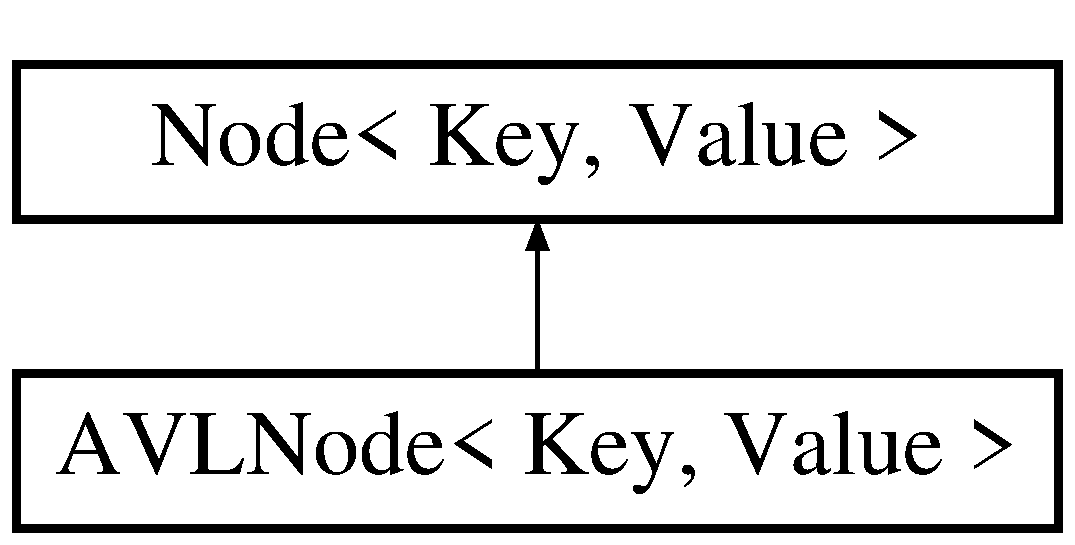
\includegraphics[height=2.000000cm]{classNode}
\end{center}
\end{figure}
\subsection*{Public Member Functions}
\begin{DoxyCompactItemize}
\item 
\hyperlink{classNode_ac9bdc0036be15ac4b622696c804c501f}{Node} (const Key \&key, const Value \&value, \hyperlink{classNode}{Node}$<$ Key, Value $>$ $\ast$parent)
\item 
virtual \hyperlink{classNode_aaa753148a7bac7330974f1a9bc9249f1}{$\sim$\-Node} ()
\item 
const std\-::pair$<$ Key, Value $>$ \& \hyperlink{classNode_a09f9422272855f3583839846de472955}{get\-Item} () const 
\item 
std\-::pair$<$ Key, Value $>$ \& \hyperlink{classNode_a70d9c3ef40626b812c9c269deeada095}{get\-Item} ()
\item 
const Key \& \hyperlink{classNode_af3cf68af83ff64ae1e947e433a57b92b}{get\-Key} () const 
\item 
const Value \& \hyperlink{classNode_a64a6ad9046786cf75f7005cfd71385e2}{get\-Value} () const 
\item 
Key \& \hyperlink{classNode_a0c782e141b79c6cb09898bbf191b2baf}{get\-Key} ()
\item 
Value \& \hyperlink{classNode_abdbbc3b9627d1bfe2106c2000d410811}{get\-Value} ()
\item 
virtual \hyperlink{classNode}{Node}$<$ Key, Value $>$ $\ast$ \hyperlink{classNode_a89780f3166c5d3aad0bd2960ce65f7a8}{get\-Parent} () const 
\item 
virtual \hyperlink{classNode}{Node}$<$ Key, Value $>$ $\ast$ \hyperlink{classNode_a2c142346d13ce08214ebee5ab76fbf72}{get\-Left} () const 
\item 
virtual \hyperlink{classNode}{Node}$<$ Key, Value $>$ $\ast$ \hyperlink{classNode_ae9aabb17b3555af256dc9ae091c0bb39}{get\-Right} () const 
\item 
void \hyperlink{classNode_a981799e30e7649812c2ad3a2d43c3f94}{set\-Parent} (\hyperlink{classNode}{Node}$<$ Key, Value $>$ $\ast$parent)
\item 
void \hyperlink{classNode_af0a4ecd342adca0c1db88f0811ad0068}{set\-Left} (\hyperlink{classNode}{Node}$<$ Key, Value $>$ $\ast$left)
\item 
void \hyperlink{classNode_ade5c16875afa559250c7a49d56007685}{set\-Right} (\hyperlink{classNode}{Node}$<$ Key, Value $>$ $\ast$right)
\item 
void \hyperlink{classNode_ab9b9a0da6a6b481623a3d1a7de5594a9}{set\-Value} (const Value \&value)
\end{DoxyCompactItemize}
\subsection*{Protected Attributes}
\begin{DoxyCompactItemize}
\item 
\hypertarget{classNode_a1f60ff1e9aa3e67b36fae39e73bd3ad0}{std\-::pair$<$ Key, Value $>$ {\bfseries m\-Item}}\label{classNode_a1f60ff1e9aa3e67b36fae39e73bd3ad0}

\item 
\hypertarget{classNode_a0edda9f5ea45078bef125a1298de9bef}{\hyperlink{classNode}{Node}$<$ Key, Value $>$ $\ast$ {\bfseries m\-Parent}}\label{classNode_a0edda9f5ea45078bef125a1298de9bef}

\item 
\hypertarget{classNode_a93b44cfd9f890e4ac24b84bb4c06b68d}{\hyperlink{classNode}{Node}$<$ Key, Value $>$ $\ast$ {\bfseries m\-Left}}\label{classNode_a93b44cfd9f890e4ac24b84bb4c06b68d}

\item 
\hypertarget{classNode_a3698d0c83982838834bc2218b15d7013}{\hyperlink{classNode}{Node}$<$ Key, Value $>$ $\ast$ {\bfseries m\-Right}}\label{classNode_a3698d0c83982838834bc2218b15d7013}

\end{DoxyCompactItemize}


\subsection{Detailed Description}
\subsubsection*{template$<$typename Key, typename Value$>$class Node$<$ Key, Value $>$}

A templated class for a \hyperlink{classNode}{Node} in a search tree. This represents a node in a normal binary search tree, but can also be extended in the future for other kinds of search trees, such as Red Black trees, Splay trees, and A\-V\-L trees. You do N\-O\-T need to implement any functionality or add additional data members or helper functions. 

\subsection{Constructor \& Destructor Documentation}
\hypertarget{classNode_ac9bdc0036be15ac4b622696c804c501f}{\index{Node@{Node}!Node@{Node}}
\index{Node@{Node}!Node@{Node}}
\subsubsection[{Node}]{\setlength{\rightskip}{0pt plus 5cm}template$<$typename Key, typename Value$>$ {\bf Node}$<$ Key, Value $>$\-::{\bf Node} (
\begin{DoxyParamCaption}
\item[{const Key \&}]{key, }
\item[{const Value \&}]{value, }
\item[{{\bf Node}$<$ Key, Value $>$ $\ast$}]{parent}
\end{DoxyParamCaption}
)}}\label{classNode_ac9bdc0036be15ac4b622696c804c501f}
Explicit constructor for a node. \hypertarget{classNode_aaa753148a7bac7330974f1a9bc9249f1}{\index{Node@{Node}!$\sim$\-Node@{$\sim$\-Node}}
\index{$\sim$\-Node@{$\sim$\-Node}!Node@{Node}}
\subsubsection[{$\sim$\-Node}]{\setlength{\rightskip}{0pt plus 5cm}template$<$typename Key , typename Value $>$ {\bf Node}$<$ Key, Value $>$\-::$\sim${\bf Node} (
\begin{DoxyParamCaption}
{}
\end{DoxyParamCaption}
)\hspace{0.3cm}{\ttfamily [virtual]}}}\label{classNode_aaa753148a7bac7330974f1a9bc9249f1}
Destructor, which does not need to do anything since the pointers inside of a node are only used as references to existing nodes. The nodes pointed to by parent/left/right are freed within the delete\-All() helper method in the \hyperlink{classBinarySearchTree}{Binary\-Search\-Tree}. 

\subsection{Member Function Documentation}
\hypertarget{classNode_a09f9422272855f3583839846de472955}{\index{Node@{Node}!get\-Item@{get\-Item}}
\index{get\-Item@{get\-Item}!Node@{Node}}
\subsubsection[{get\-Item}]{\setlength{\rightskip}{0pt plus 5cm}template$<$typename Key , typename Value $>$ const std\-::pair$<$ Key, Value $>$ \& {\bf Node}$<$ Key, Value $>$\-::get\-Item (
\begin{DoxyParamCaption}
{}
\end{DoxyParamCaption}
) const}}\label{classNode_a09f9422272855f3583839846de472955}
A const getter for the item. \hypertarget{classNode_a70d9c3ef40626b812c9c269deeada095}{\index{Node@{Node}!get\-Item@{get\-Item}}
\index{get\-Item@{get\-Item}!Node@{Node}}
\subsubsection[{get\-Item}]{\setlength{\rightskip}{0pt plus 5cm}template$<$typename Key , typename Value $>$ std\-::pair$<$ Key, Value $>$ \& {\bf Node}$<$ Key, Value $>$\-::get\-Item (
\begin{DoxyParamCaption}
{}
\end{DoxyParamCaption}
)}}\label{classNode_a70d9c3ef40626b812c9c269deeada095}
A non-\/const getter for the item. \hypertarget{classNode_af3cf68af83ff64ae1e947e433a57b92b}{\index{Node@{Node}!get\-Key@{get\-Key}}
\index{get\-Key@{get\-Key}!Node@{Node}}
\subsubsection[{get\-Key}]{\setlength{\rightskip}{0pt plus 5cm}template$<$typename Key , typename Value $>$ const Key \& {\bf Node}$<$ Key, Value $>$\-::get\-Key (
\begin{DoxyParamCaption}
{}
\end{DoxyParamCaption}
) const}}\label{classNode_af3cf68af83ff64ae1e947e433a57b92b}
A const getter for the key. \hypertarget{classNode_a0c782e141b79c6cb09898bbf191b2baf}{\index{Node@{Node}!get\-Key@{get\-Key}}
\index{get\-Key@{get\-Key}!Node@{Node}}
\subsubsection[{get\-Key}]{\setlength{\rightskip}{0pt plus 5cm}template$<$typename Key , typename Value $>$ Key \& {\bf Node}$<$ Key, Value $>$\-::get\-Key (
\begin{DoxyParamCaption}
{}
\end{DoxyParamCaption}
)}}\label{classNode_a0c782e141b79c6cb09898bbf191b2baf}
A non-\/const getter for the key. \hypertarget{classNode_a2c142346d13ce08214ebee5ab76fbf72}{\index{Node@{Node}!get\-Left@{get\-Left}}
\index{get\-Left@{get\-Left}!Node@{Node}}
\subsubsection[{get\-Left}]{\setlength{\rightskip}{0pt plus 5cm}template$<$typename Key , typename Value $>$ {\bf Node}$<$ Key, Value $>$ $\ast$ {\bf Node}$<$ Key, Value $>$\-::get\-Left (
\begin{DoxyParamCaption}
{}
\end{DoxyParamCaption}
) const\hspace{0.3cm}{\ttfamily [virtual]}}}\label{classNode_a2c142346d13ce08214ebee5ab76fbf72}
An implementation of the virtual function for retreiving the left child. 

Reimplemented in \hyperlink{classAVLNode_af681acf83cebd11fb1083262b8100c70}{A\-V\-L\-Node$<$ Key, Value $>$}.

\hypertarget{classNode_a89780f3166c5d3aad0bd2960ce65f7a8}{\index{Node@{Node}!get\-Parent@{get\-Parent}}
\index{get\-Parent@{get\-Parent}!Node@{Node}}
\subsubsection[{get\-Parent}]{\setlength{\rightskip}{0pt plus 5cm}template$<$typename Key , typename Value $>$ {\bf Node}$<$ Key, Value $>$ $\ast$ {\bf Node}$<$ Key, Value $>$\-::get\-Parent (
\begin{DoxyParamCaption}
{}
\end{DoxyParamCaption}
) const\hspace{0.3cm}{\ttfamily [virtual]}}}\label{classNode_a89780f3166c5d3aad0bd2960ce65f7a8}
An implementation of the virtual function for retreiving the parent. 

Reimplemented in \hyperlink{classAVLNode_a192664222857753573eba15c6e9b6205}{A\-V\-L\-Node$<$ Key, Value $>$}.

\hypertarget{classNode_ae9aabb17b3555af256dc9ae091c0bb39}{\index{Node@{Node}!get\-Right@{get\-Right}}
\index{get\-Right@{get\-Right}!Node@{Node}}
\subsubsection[{get\-Right}]{\setlength{\rightskip}{0pt plus 5cm}template$<$typename Key , typename Value $>$ {\bf Node}$<$ Key, Value $>$ $\ast$ {\bf Node}$<$ Key, Value $>$\-::get\-Right (
\begin{DoxyParamCaption}
{}
\end{DoxyParamCaption}
) const\hspace{0.3cm}{\ttfamily [virtual]}}}\label{classNode_ae9aabb17b3555af256dc9ae091c0bb39}
An implementation of the virtual function for retreiving the right child. 

Reimplemented in \hyperlink{classAVLNode_ac57cebda2c1b448d22e00dcb9248cfb8}{A\-V\-L\-Node$<$ Key, Value $>$}.

\hypertarget{classNode_a64a6ad9046786cf75f7005cfd71385e2}{\index{Node@{Node}!get\-Value@{get\-Value}}
\index{get\-Value@{get\-Value}!Node@{Node}}
\subsubsection[{get\-Value}]{\setlength{\rightskip}{0pt plus 5cm}template$<$typename Key , typename Value $>$ const Value \& {\bf Node}$<$ Key, Value $>$\-::get\-Value (
\begin{DoxyParamCaption}
{}
\end{DoxyParamCaption}
) const}}\label{classNode_a64a6ad9046786cf75f7005cfd71385e2}
A const getter for the value. \hypertarget{classNode_abdbbc3b9627d1bfe2106c2000d410811}{\index{Node@{Node}!get\-Value@{get\-Value}}
\index{get\-Value@{get\-Value}!Node@{Node}}
\subsubsection[{get\-Value}]{\setlength{\rightskip}{0pt plus 5cm}template$<$typename Key , typename Value $>$ Value \& {\bf Node}$<$ Key, Value $>$\-::get\-Value (
\begin{DoxyParamCaption}
{}
\end{DoxyParamCaption}
)}}\label{classNode_abdbbc3b9627d1bfe2106c2000d410811}
A non-\/const getter for the value. \hypertarget{classNode_af0a4ecd342adca0c1db88f0811ad0068}{\index{Node@{Node}!set\-Left@{set\-Left}}
\index{set\-Left@{set\-Left}!Node@{Node}}
\subsubsection[{set\-Left}]{\setlength{\rightskip}{0pt plus 5cm}template$<$typename Key, typename Value$>$ void {\bf Node}$<$ Key, Value $>$\-::set\-Left (
\begin{DoxyParamCaption}
\item[{{\bf Node}$<$ Key, Value $>$ $\ast$}]{left}
\end{DoxyParamCaption}
)}}\label{classNode_af0a4ecd342adca0c1db88f0811ad0068}
A setter for setting the left child of a node. \hypertarget{classNode_a981799e30e7649812c2ad3a2d43c3f94}{\index{Node@{Node}!set\-Parent@{set\-Parent}}
\index{set\-Parent@{set\-Parent}!Node@{Node}}
\subsubsection[{set\-Parent}]{\setlength{\rightskip}{0pt plus 5cm}template$<$typename Key, typename Value$>$ void {\bf Node}$<$ Key, Value $>$\-::set\-Parent (
\begin{DoxyParamCaption}
\item[{{\bf Node}$<$ Key, Value $>$ $\ast$}]{parent}
\end{DoxyParamCaption}
)}}\label{classNode_a981799e30e7649812c2ad3a2d43c3f94}
A setter for setting the parent of a node. \hypertarget{classNode_ade5c16875afa559250c7a49d56007685}{\index{Node@{Node}!set\-Right@{set\-Right}}
\index{set\-Right@{set\-Right}!Node@{Node}}
\subsubsection[{set\-Right}]{\setlength{\rightskip}{0pt plus 5cm}template$<$typename Key, typename Value$>$ void {\bf Node}$<$ Key, Value $>$\-::set\-Right (
\begin{DoxyParamCaption}
\item[{{\bf Node}$<$ Key, Value $>$ $\ast$}]{right}
\end{DoxyParamCaption}
)}}\label{classNode_ade5c16875afa559250c7a49d56007685}
A setter for setting the right child of a node. \hypertarget{classNode_ab9b9a0da6a6b481623a3d1a7de5594a9}{\index{Node@{Node}!set\-Value@{set\-Value}}
\index{set\-Value@{set\-Value}!Node@{Node}}
\subsubsection[{set\-Value}]{\setlength{\rightskip}{0pt plus 5cm}template$<$typename Key , typename Value$>$ void {\bf Node}$<$ Key, Value $>$\-::set\-Value (
\begin{DoxyParamCaption}
\item[{const Value \&}]{value}
\end{DoxyParamCaption}
)}}\label{classNode_ab9b9a0da6a6b481623a3d1a7de5594a9}
A setter for the value of a node. 

The documentation for this class was generated from the following file\-:\begin{DoxyCompactItemize}
\item 
bst.\-h\end{DoxyCompactItemize}

\hypertarget{structRectangle}{\section{Rectangle Struct Reference}
\label{structRectangle}\index{Rectangle@{Rectangle}}
}
\subsection*{Public Attributes}
\begin{DoxyCompactItemize}
\item 
\hypertarget{structRectangle_acb6f320ca8716ad841f0e8c7c032cd25}{int {\bfseries I\-D}}\label{structRectangle_acb6f320ca8716ad841f0e8c7c032cd25}

\item 
\hypertarget{structRectangle_ae59ba4b220bd28539821b64b48553b75}{int {\bfseries length}}\label{structRectangle_ae59ba4b220bd28539821b64b48553b75}

\item 
\hypertarget{structRectangle_ac564db1ed0dd61dd82a5276399bc72ad}{int {\bfseries height}}\label{structRectangle_ac564db1ed0dd61dd82a5276399bc72ad}

\end{DoxyCompactItemize}


The documentation for this struct was generated from the following file\-:\begin{DoxyCompactItemize}
\item 
floorplan.\-cpp\end{DoxyCompactItemize}

\hypertarget{classTreeTest}{\section{Tree\-Test Class Reference}
\label{classTreeTest}\index{Tree\-Test@{Tree\-Test}}
}
Inheritance diagram for Tree\-Test\-:\begin{figure}[H]
\begin{center}
\leavevmode
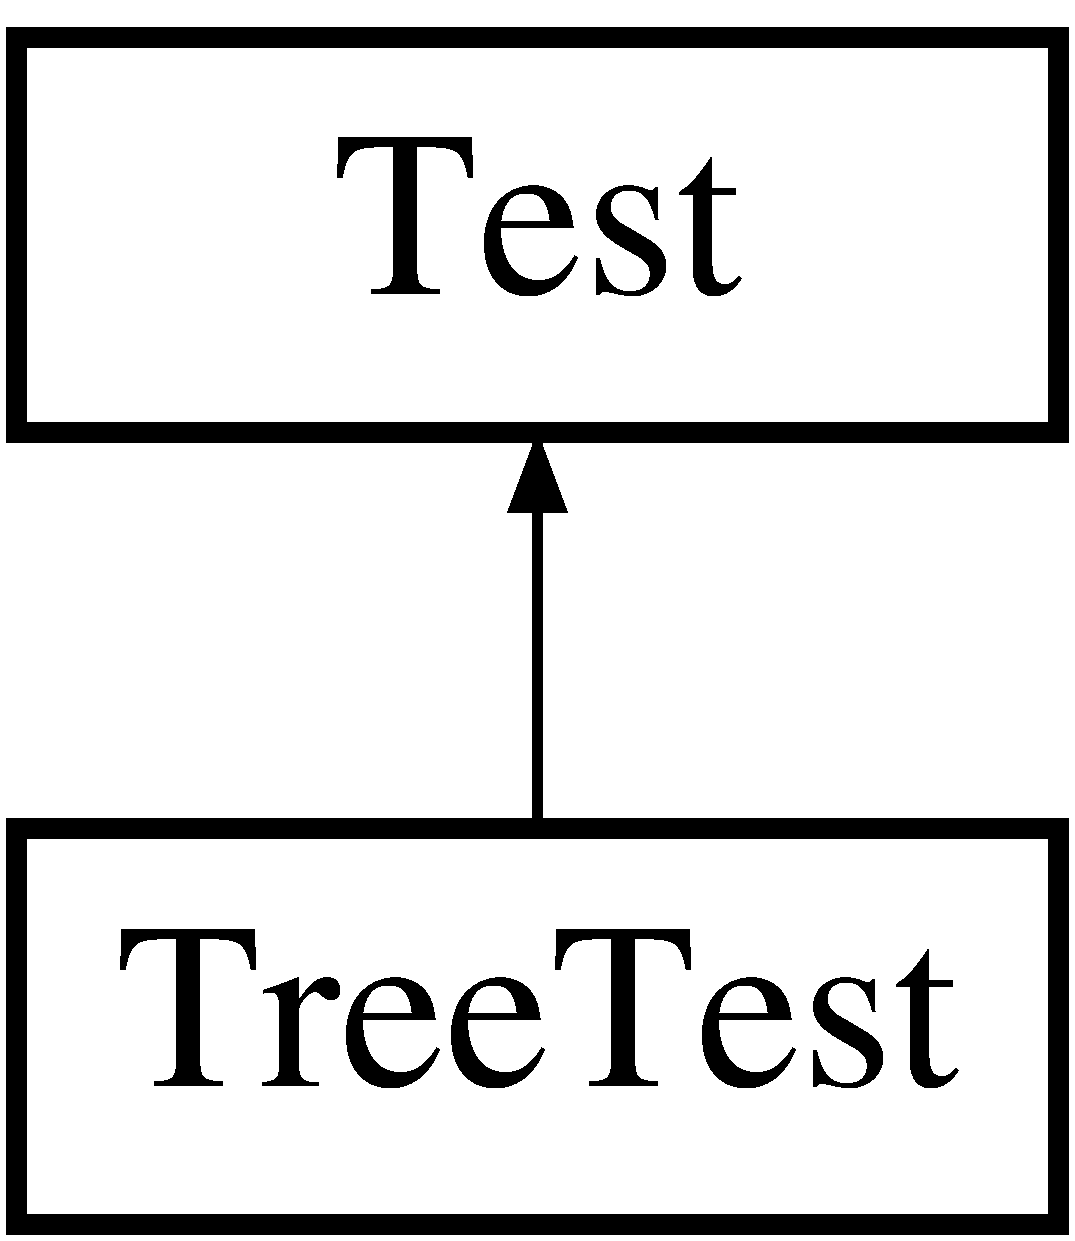
\includegraphics[height=2.000000cm]{classTreeTest}
\end{center}
\end{figure}
\subsection*{Protected Member Functions}
\begin{DoxyCompactItemize}
\item 
\hypertarget{classTreeTest_a50caa23d3a9be5549c5b26fe78412602}{virtual void {\bfseries Set\-Up} ()}\label{classTreeTest_a50caa23d3a9be5549c5b26fe78412602}

\item 
\hypertarget{classTreeTest_af62231881288188320962c123d9c1629}{virtual void {\bfseries Tear\-Down} ()}\label{classTreeTest_af62231881288188320962c123d9c1629}

\end{DoxyCompactItemize}
\subsection*{Protected Attributes}
\begin{DoxyCompactItemize}
\item 
\hypertarget{classTreeTest_aaba2ba8609158514d6aad8f2df60a448}{\hyperlink{classBinarySearchTree}{Binary\-Search\-Tree}$<$ int, int $>$ {\bfseries bst1}}\label{classTreeTest_aaba2ba8609158514d6aad8f2df60a448}

\end{DoxyCompactItemize}


The documentation for this class was generated from the following file\-:\begin{DoxyCompactItemize}
\item 
tree\-Test.\-cpp\end{DoxyCompactItemize}

%--- End generated contents ---

% Index
\newpage
\phantomsection
\addcontentsline{toc}{chapter}{Index}
\printindex

\end{document}
